\documentclass[11pt, a4paper]{article}

\usepackage[utf8]{inputenc}
\usepackage{geometry}
\geometry{a4paper, margin=1in}
\usepackage{hyperref}
\usepackage{graphicx}
\usepackage{booktabs}
\usepackage{tabularx}
\usepackage{enumitem}
\usepackage{tikz}
\usetikzlibrary{shapes.geometric, arrows.meta, positioning, fit, backgrounds}

\title{\textbf{Comprehensive Report: End-to-End Skill Extraction \& Dataset Generation Pipeline}}
\author{Data Engineering \& NLP Research Team}
\date{\today}

\begin{document}

\maketitle

\begin{abstract}
This document details the architecture and implementation of an end-to-end data pipeline designed to harvest live job postings and transform them into a high-quality, sequence-labeling dataset for Named Entity Recognition (NER). The project comprises two major subsystems: an asynchronous, ATS-aware web scraping engine, and a 12-phase natural language processing (NLP) transformation pipeline. The final output is a silver-standard dataset tailored for training models on exact skill span extraction, formatted in the industry-standard CoNLL format with BIO tags for \texttt{hard\_skill} and \texttt{soft\_skill} categories.
\end{abstract}

\tableofcontents
\newpage

\section{Introduction}
As the demand for precise skill extraction from job postings grows, training robust sequence-labeling models becomes paramount. The objective of this project was twofold:
\begin{enumerate}
    \item \textbf{Data Acquisition:} Develop a robust scraping engine capable of parsing diverse GitHub repositories (e.g., SpeedyApply, intern-intl) and navigating complex Applicant Tracking Systems (ATS) like Workday, Greenhouse, and Lever to extract full-text job descriptions.
    \item \textbf{Dataset Transformation:} Convert the raw, heterogeneous scraped data into a structured, trainable sequence-labeling dataset that strictly adheres to exact substring matching, preventing hallucinated skills, and providing standard train/dev/test splits.
\end{enumerate}

\section{System Architecture}

The system is logically separated into the Extraction Engine and the Dataset Transformation Pipeline.

\begin{figure}[h]
\centering
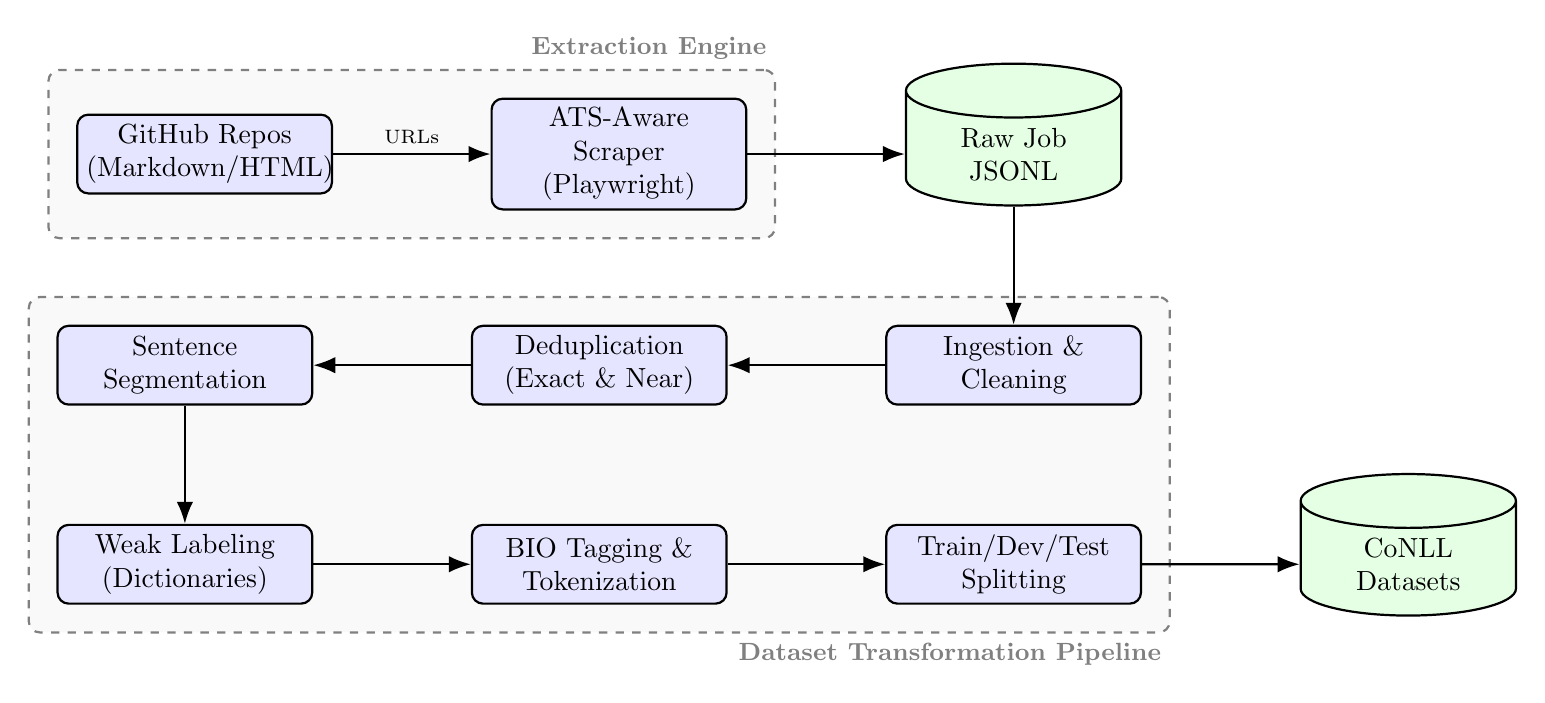
\begin{tikzpicture}[
    node distance=1.5cm and 2cm,
    box/.style={rectangle, draw=black, thick, fill=blue!10, text width=3cm, align=center, rounded corners, minimum height=1cm},
    data/.style={cylinder, draw=black, thick, fill=green!10, text width=2.5cm, align=center, shape border rotate=90, aspect=0.25, minimum height=1.2cm},
    arrow/.style={-{Latex[scale=1.2]}, thick}
]

% Extraction Phase
\node[box] (github) {GitHub Repos\\(Markdown/HTML)};
\node[box, right=of github] (scraper) {ATS-Aware\\Scraper (Playwright)};
\node[data, right=of scraper] (rawdata) {Raw Job\\JSONL};

\draw[arrow] (github) -- node[above, text width=2cm, align=center, font=\scriptsize] {URLs} (scraper);
\draw[arrow] (scraper) -- (rawdata);

% Background box for Extraction
\begin{scope}[on background layer]
    \node[draw=gray, dashed, thick, rounded corners, fill=gray!5, fit=(github)(scraper), inner sep=10pt] (extract_box) {};
    \node[above left, font=\bfseries\small, text=gray] at (extract_box.north east) {Extraction Engine};
\end{scope}

% Transformation Phase
\node[box, below=of rawdata] (ingest) {Ingestion \&\\Cleaning};
\node[box, left=of ingest] (dedup) {Deduplication\\(Exact \& Near)};
\node[box, left=of dedup] (segment) {Sentence\\Segmentation};
\node[box, below=of segment] (weak) {Weak Labeling\\(Dictionaries)};
\node[box, right=of weak] (bio) {BIO Tagging \&\\Tokenization};
\node[box, right=of bio] (split) {Train/Dev/Test\\Splitting};
\node[data, right=of split] (final) {CoNLL\\Datasets};

\draw[arrow] (rawdata) -- (ingest);
\draw[arrow] (ingest) -- (dedup);
\draw[arrow] (dedup) -- (segment);
\draw[arrow] (segment) -- (weak);
\draw[arrow] (weak) -- (bio);
\draw[arrow] (bio) -- (split);
\draw[arrow] (split) -- (final);

% Background box for Pipeline
\begin{scope}[on background layer]
    \node[draw=gray, dashed, thick, rounded corners, fill=gray!5, fit=(ingest)(dedup)(segment)(weak)(bio)(split), inner sep=10pt] (transform_box) {};
    \node[below left, font=\bfseries\small, text=gray] at (transform_box.south east) {Dataset Transformation Pipeline};
\end{scope}

\end{tikzpicture}
\caption{End-to-End System Architecture Pipeline}
\label{fig:arch}
\end{figure}

\newpage
\section{Part 1: The Extraction Engine}

The data acquisition phase relies on a custom-built, asynchronous Python scraping engine designed to handle the dynamic nature of modern job portals.

\subsection{Source Parsing (\texttt{scraper/github\_sources.py})}
The entry point of the scraper involves parsing curated lists of job postings hosted on GitHub. Because repositories format their data differently, we implemented robust parsers:
\begin{itemize}
    \item \textbf{HTML Tables:} Utilized \texttt{BeautifulSoup} to parse complex \texttt{<table>} elements.
    \item \textbf{Markdown Tables:} Implemented custom pipe-delimited regex parsers to cleanly extract company names, roles, and application URLs from repositories like \texttt{SpeedyApply} and \texttt{intern\_intl}.
\end{itemize}

\subsection{ATS Detection and Navigation (\texttt{scraper/detectors.py} \& \texttt{extractor.py})}
Once URLs are extracted, the engine must navigate the target sites. 
\begin{itemize}
    \item \textbf{Heuristic Detection:} The system analyzes URL patterns (e.g., \texttt{myworkdayjobs.com}, \texttt{boards.greenhouse.io}) to identify the underlying ATS provider.
    \item \textbf{Dynamic Interaction:} Using \texttt{Playwright}, the engine performs asynchronous, headless browser automation. It intelligently handles dynamic UI elements, such as clicking "See More" buttons or closing cookie consent popups, ensuring the entire text of the job description is loaded into the DOM before extraction.
\end{itemize}

\subsection{State Management (\texttt{scraper/utils.py})}
To support highly concurrent runs and gracefully handle network interruptions, the engine implements continuous state checkpointing via a CSV tracker. Extracted records are incrementally appended to \texttt{data/raw/job\_descriptions.jsonl}.

\section{Part 2: The Dataset Transformation Pipeline}

The core contribution of this project is the 12-phase transformation pipeline that converts the raw HTML/text descriptions into a structured machine-learning dataset.

\subsection{Phase 1: Ingestion and Normalization (\texttt{src/ingest/ingest.py})}
Because data can arrive in various formats (CSV, JSON, JSONL), the ingestion module reads from the \texttt{data/raw} directory and maps all entries to a strictly enforced internal schema. Fields include a deterministic \texttt{job\_id} (hashed from the URL and title), \texttt{company}, \texttt{location}, and the \texttt{raw\_text}.

\subsection{Phase 2: Cleaning (\texttt{src/clean/clean.py})}
Raw job descriptions often contain heavy HTML boilerplate. The cleaning module strips all HTML tags using \texttt{BeautifulSoup}. Crucially, while erratic whitespace is normalized, all sentence-ending punctuation is strictly preserved. This is vital, as removing punctuation would irreversibly damage downstream sentence boundary detection.

\subsection{Phase 3: Deduplication (\texttt{src/dedup/dedup.py})}
Companies frequently re-post identical jobs, which can artificially inflate test-set performance (data leakage) if not handled. We implemented a two-tiered deduplication strategy:
\begin{enumerate}
    \item \textbf{Exact Matches:} Utilized MD5 hashing on the cleaned text to drop perfect replicas.
    \item \textbf{Near-Duplicates:} Employed a Jaccard similarity threshold over word sets to identify and remove postings that only differ by minor formatting or updated timestamps.
\end{enumerate}
This phase successfully filtered out 338 duplicates, reducing the corpus from 1,887 to 1,549 unique postings.

\subsection{Phase 4: Sentence Segmentation (\texttt{src/segment/segment.py})}
To prepare the text for sequence modeling, the descriptions must be split into sentences. The module uses robust regular expressions (\texttt{[\textasciicircum.!?]*[.!?]}) to find sentence boundaries. A critical feature of this module is its ability to map the exact character \texttt{start} and \texttt{end} indices of every sentence back to the original document, ensuring traceability. This phase produced over 90,000 individual sentences.

\subsection{Phase 5 \& 6: Weak Labeling (\texttt{src/weak\_label/weak\_label.py})}
To create a "silver" (machine-generated but highly accurate) dataset without manual annotation, we implemented a dictionary-based weak labeling engine. 
\begin{itemize}
    \item \textbf{Dictionaries:} We curated extensive lists of \texttt{hard\_skill} terms (e.g., Python, Kubernetes, TensorFlow) and \texttt{soft\_skill} terms (e.g., Leadership, Communication).
    \item \textbf{Extraction:} The engine performs word-boundary regular expression matching against the sentences. When a match occurs, the system records the exact substring, the label type, the start/end indices, and assigns a confidence score.
\end{itemize}

\subsection{Phase 7: BIO Tagging and Tokenization (\texttt{src/convert/convert\_to\_bio.py})}
Sequence labeling models (like BERT-CRF) require text to be tokenized and tagged using the BIO (Begin, Inside, Outside) format.
\begin{itemize}
    \item The sentence is tokenized on whitespace and punctuation.
    \item The character-level spans from Phase 6 are projected onto the tokens. The first token of a skill receives a \texttt{B-} prefix (e.g., \texttt{B-hard\_skill}), subsequent tokens receive \texttt{I-}, and non-skill tokens receive \texttt{O}.
\end{itemize}

\subsection{Phase 8 \& 10: Validation and Gold Review (\texttt{validate/})}
Data integrity is enforced through a strict validation script (\texttt{validate.py}) that computationally checks invariants:
\begin{enumerate}
    \item The substring sliced using the recorded indices must perfectly match the reported span text.
    \item The length of the token array must exactly equal the length of the NER tag array.
\end{enumerate}
The pipeline achieved a 100\% pass rate across all 90,220 sentences. Additionally, a randomized 100-record subset was exported to CSV (\texttt{prepare\_gold.py}) to serve as a template for human annotators to construct a pristine Gold test set.

\subsection{Phase 9: Data Splitting (\texttt{src/split/split.py})}
To evaluate models effectively, the data is split into Train (70\%), Dev (15\%), and Test (15\%) sets. \textbf{Crucially, this split is performed at the \texttt{job\_id} level, not the sentence level.} If split by sentence, similar bullet points from the same job description might end up in both the Train and Test sets, causing massive data leakage. The output is saved in both JSONL and standard CoNLL formats.

\subsection{Phase 11: Dataset Statistics (\texttt{src/stats/stats.py})}
The pipeline concludes by calculating comprehensive summary statistics regarding skill distributions, average sentence lengths, and span densities, which are critical for understanding the domain distribution prior to model training.

\section{Dataset Results \& Statistics}
The pipeline processed 1,549 unique jobs into 90,220 sentences. Of these, 7,493 sentences were identified as containing at least one labeled skill, yielding 7,550 hard skills and 4,524 soft skills.

\begin{table}[h]
\centering
\caption{Most Common Extracted Skills across the Dataset}
\begin{tabular}{lr | lr}
\toprule
\textbf{Hard Skill} & \textbf{Count} & \textbf{Soft Skill} & \textbf{Count} \\
\midrule
Python & 1,117 & Communication & 1,098 \\
Machine Learning & 1,064 & Collaboration & 646 \\
Data Science & 726 & Creativity & 569 \\
SQL & 497 & Organization & 525 \\
Data Analysis & 383 & Leadership & 385 \\
Java & 307 & Agile & 293 \\
AWS & 302 & Attention to Detail & 179 \\
Deep Learning & 258 & Teamwork & 153 \\
Azure & 218 & Project Management & 132 \\
HTML & 193 & Problem Solving & 118 \\
\bottomrule
\end{tabular}
\end{table}

\section{Conclusion and Future Work}
The constructed system represents a robust, production-grade data engineering pipeline that seamlessly connects raw web data acquisition with rigorous NLP dataset formulation. By ensuring exact character alignments, preventing data leakage through job-level splitting, and producing CoNLL-formatted outputs, the dataset is immediately ready for training state-of-the-art transformer models.

\textbf{Future Work:}
While dictionary-based weak labeling provides a strong silver baseline, it fails to capture highly contextual, multi-word skills (e.g., "ability to design scalable microservices"). Future iterations will integrate Large Language Models (LLMs) into the weak labeling phase to generate higher-fidelity, context-aware annotations, further closing the gap between the silver dataset and human-annotated gold standards.

\end{document}
